

\newpage
\begin{center}
    \textbf{\large 4. FLUTTER ПРИЛОЖЕНИЕ}
\end{center}
\refstepcounter{chapter}
\addcontentsline{toc}{chapter}{4. FLUTTER ПРИЛОЖЕНИЕ}

Мобильное приложение для получения расписания МТУСИ создано на базе фреймворка Flutter 
и предназначено для студентов, преподавателей и сотрудников университета. 
Пользователи могут выбрать свою группу, аудиторию, преподавателя, предмет и даты, 
на которые они хотят получить расписание занятий и экзаменов. 
После выбора фильтров, приложение обращается к GraphQL API, чтобы получить данные о занятиях и экзаменах, 
соответствующих заданным фильтрам.

Приложение имеет удобный интерфейс, который позволяет просматривать расписание. 
Кроме того, приложение позволяет экспортировать расписание в формате ICS, и добавлять в календарь.
Для удобства использования приложение имеет функции быстрого поиска и фильтрации,
которые позволяют пользователям быстро находить нужную информацию.
Кроме того, приложение сохраняет последний запрос в кеше устройства,
чтобы пользователи могли быстро вернуться к предыдущим поискам.

Мобильное приложение для получения расписания МТУСИ является удобным и
эффективным инструментом для студентов, преподавателей и сотрудников университета,
которые хотят быть в курсе своего расписания занятий и экзаменов.

\section{Обзор технологий, использованных при разработке приложения}

\textbf{Flutter} --- это фреймворк для разработки мобильных приложений,
созданный компанией Google.
Он позволяет создавать высокопроизводительные приложения для Android и iOS
с использованием одного и того же кода на языке программирования Dart.
Flutter использует собственный движок для отрисовки пользовательского интерфейса,
что позволяет достичь высокой производительности и кроссплатформенной совместимости.
Flutter также предоставляет широкий набор виджетов и инструментов для создания красивого
и интуитивно понятного пользовательского интерфейса.

\textbf{Реактивный подход} --- это подход к разработке программного обеспечения,
который основан на обработке изменений данных. 
В реактивном подходе данные представляются в виде потоков,
которые изменяются во времени.
При изменении данных в потоке, происходит обновление пользовательского интерфейса.

\section{Функции приложения}
\subsection{Экран поиска}
Экран поиска является одной из ключевых функций сервиса.
Он позволяет пользователям быстро находить расписания занятий и экзаменов по различным параметрам.
Пользователи могут искать информацию по группам, преподавателям, аудиториям и предметам.
Подсказки отображаются на экране поиска в реальном времени, когда пользователь начинает вводить запрос.
Когда пользователь начинает вводить буквы, экран поиска предлагает список наиболее подходящих результатов,
основанных на уже введенных символах.
Например, если пользователь начинает вводить название группы,
экран поиска предлагает список всех групп, у которых в названии есть введенные символы.
Пользователь может выбрать нужную группу из списка и получить соответствующее расписание занятий и экзаменов.
Этот механизм упрощает и ускоряет поиск информации для пользователей,
делая сервис более удобным и эффективным.

\begin{figure}[h]
\centering
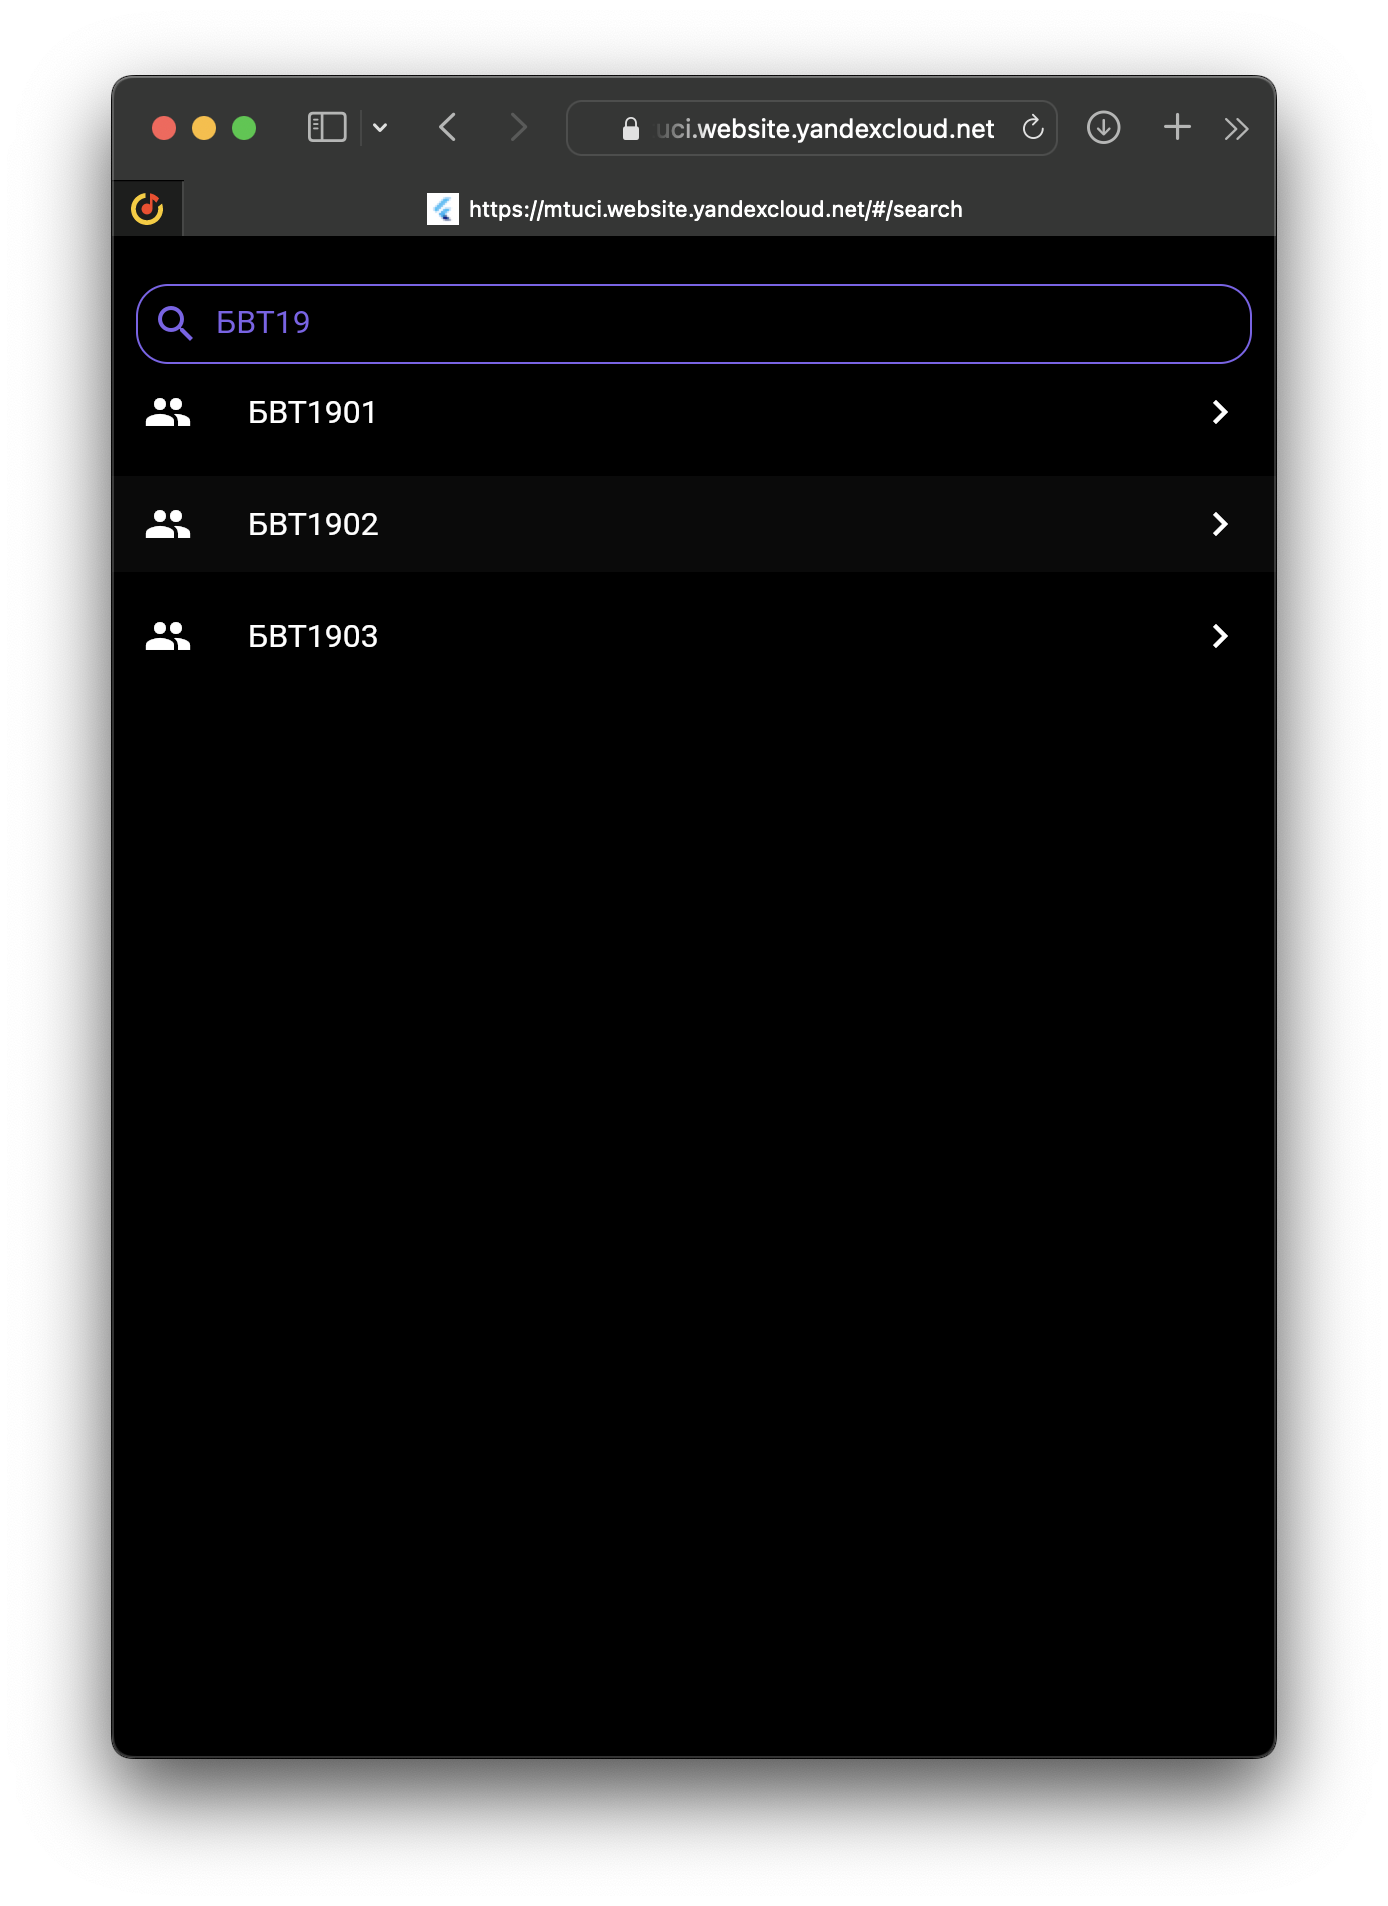
\includegraphics[width=0.8\linewidth]{images/search_screen.png}
\caption{Скриншот экрана поиска}
\label{fig:mpr}
\end{figure}